        \section{Overview of higher dimensional functions}
        Aside from the study of linear transformations on $\R^n$ or $\C^n$, we have limited ourselves to functions of a single variable.  Given that we have performed a deep analysis for functions of one variable, we can take what we have learned and apply it to new types of functions. Specifically, we will concentrate on domains in $\R^3$ (or often $\R^2$) and view functions of the form:
        \begin{align*}
            &\curvegamma\colon \R \to \R^3\\
            &f\colon \R^3 \to \R\\
            &\vecfieldV \colon \R^3 \to \R^3.
        \end{align*}
        Of these three functions, the first is called a \boldgreen{curve} \index{curve} the latter two are often referred to as \boldgreen{fields} \index{field} due to their inherent attachment to geometric objects.  These fields are also \boldgreen{multivariate} functions since their inputs depend on points in $\R^3$, whereas the first only has an input of a single variable that we typically think of as time.
        
        A point $\vecx$ in space $\R^3$, or more generally, a point in $\R^n$ is given by specifying $n$ coordinates. For example, in space we may take
        \[
        \vecx = (x,y,z) = x\xhat + y\yhat + z\zhat = \begin{pmatrix} x \\ y \\ z \end{pmatrix}.
        \]
        All of these forms of notation are equivalent in our case. The latter two were what we typically used in the prequel, but we find utility in the slightly more compact notation $(x,y,z)$ when specifying input to a function. 
        

        \begin{enumerate}[(1)]
        \item Once again, functions that assume the form
        \[
        \curvegamma \colon \R\to \R^3
        \]
        are curves. More generally, we can have a curve take input values from a restricted domain and the output can lie in an arbitrary dimension. Hence, we may put
        \[
        \curvegamma \colon [a,b]\to \R^n.
        \]
        Another specific example would be a \boldgreen{planar curve} for which we take $n=2$. Note, we can always take $a=0$ and $b=1$ to yield a planar curve 
        \[
            \curvegamma \colon [0,1] \to \R^2.
        \]
        Curves arise in many scenarios. We plot curves when we first learn about functions. We solve for curves when we find solutions to ODEs. Curves also provide a mathematician a way for exploring a space of interest. Often times we think of $\curvegamma(t)$ as describing a particle or observer's position at the time $t$.

        \begin{figure}[H]
            \centering
            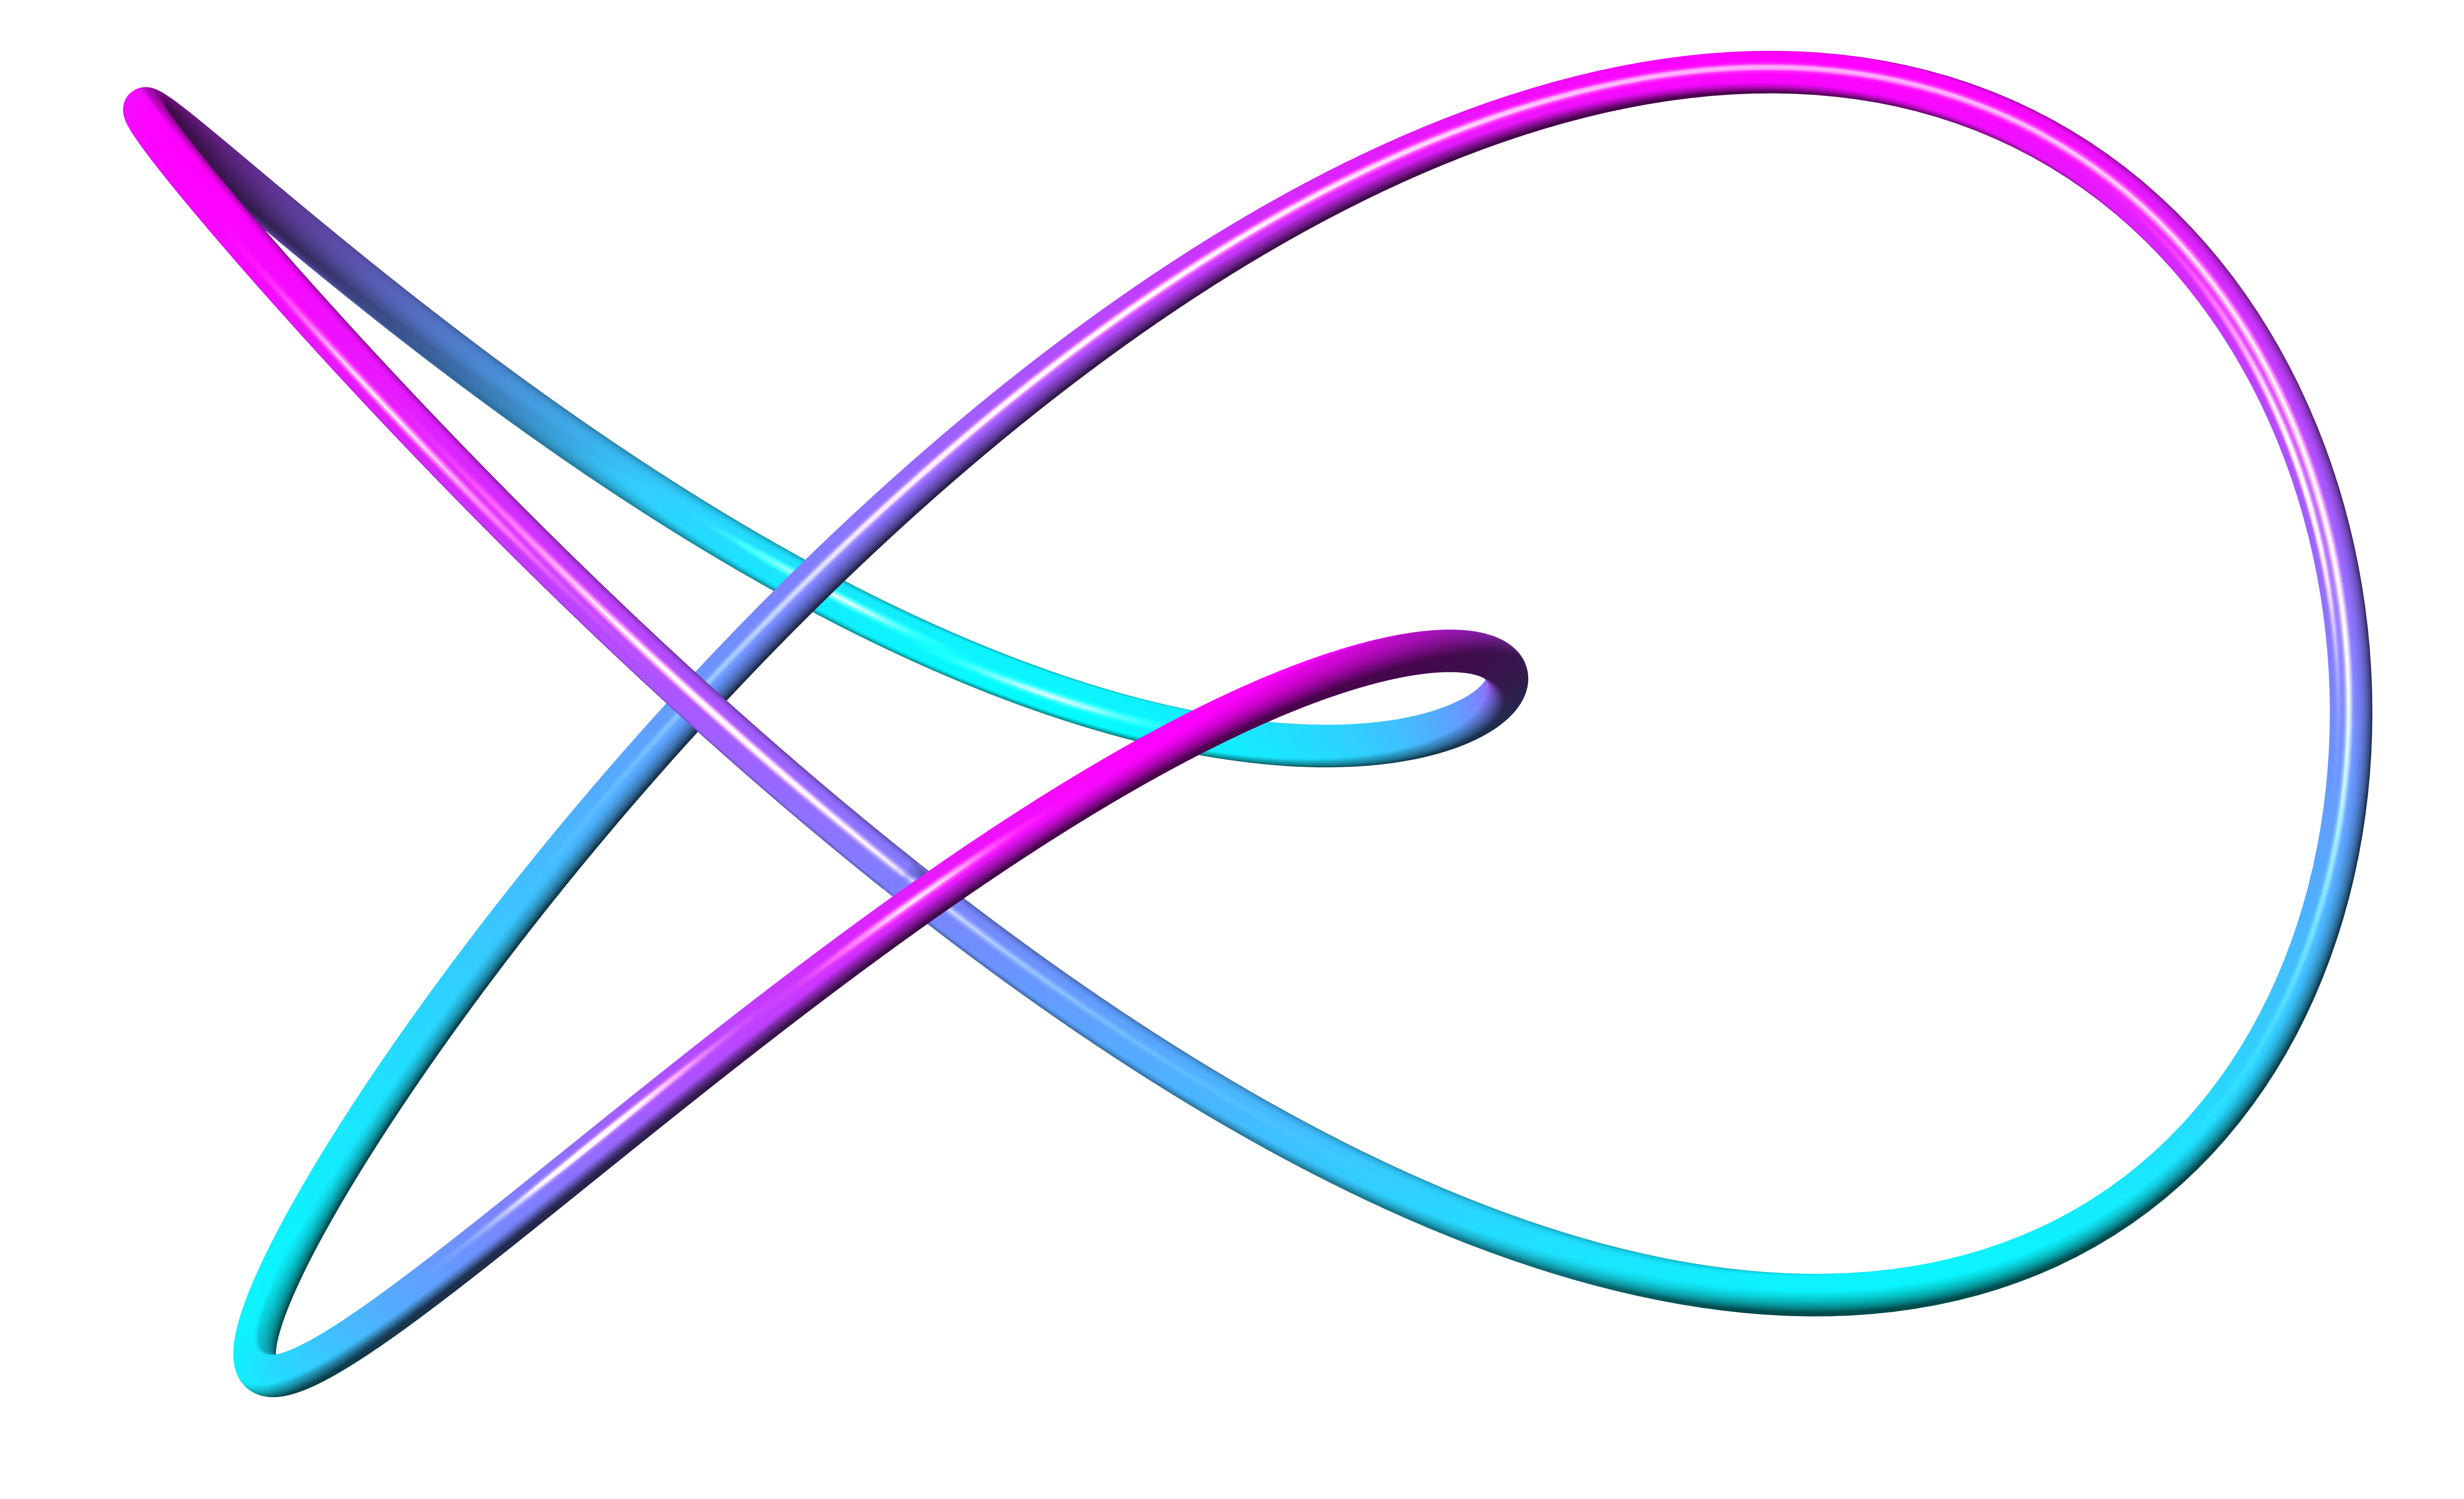
\includegraphics[width=.8\textwidth]{Figures_Part_5/trefoil_knot.png}
            \caption{A curve called the trefoil knot. Notice how the curve wraps around itself in an interesting way (notice the lighting on each portion of the curve to see these overlaps). The reader can try to recreate this curve with a string!}
        \end{figure}
        
        \item Functions of the form
        \[
        f\colon \R^3 \to \R
        \]
        are \boldgreen{scalar fields}. These types of functions are useful in describing quantities like temperature in space. In this example, at each point $\vecx=(x,y,z)$ in 3-dimensional space $\R^3$, we can assign a single real number output $f(\vecx)=f(x,y,z)$ that tells us this temperature. Or, we may find that we restrict ourselves to a specific domain $\Omega$ that lives in space. In that case, $\Omega$ may represent a physical object for which we want to describe temperature. Hence, we have
        \[
        f \colon \Omega \to \R
        \] 
        is a scalar field defined on $\Omega$. For a point $(x,y,z) \in \Omega$, the value of $f$ at that point is $f(x,y,z)$. This is where we see a slight distinction between functions and fields. Fields arise from a geometrical object (e.g., space itself or an object embedded in space). Once again, if we are thinking of $f$ as describing temperature, we may want to describe how this temperature field change over time. Abstractly, our function then assumes the form
        \[
        f \colon \Omega \times [0,\infty) \to \R,
        \]
        and the value of $f$ at $(x,y,z) \in \Omega$ and time $t$ is $f(x,y,z,t)$. We will return to the time dependent fields later as we visit Partial Differential Equations (PDEs).

        To advance our intuition of functions we have used techniques for visualization. For example, with a function $f \colon \R \to \R$ we drew the graph of the function by plotting the points $(x,f(x))$ for all values of $x$. Sadly, full visualization of 3-dimensional scalar fields would require us to visualize 4-dimensions. Many examples we will do will instead take 2-dimensional scalar functions in order to build intuition.

        \begin{figure}[H]
            \centering
            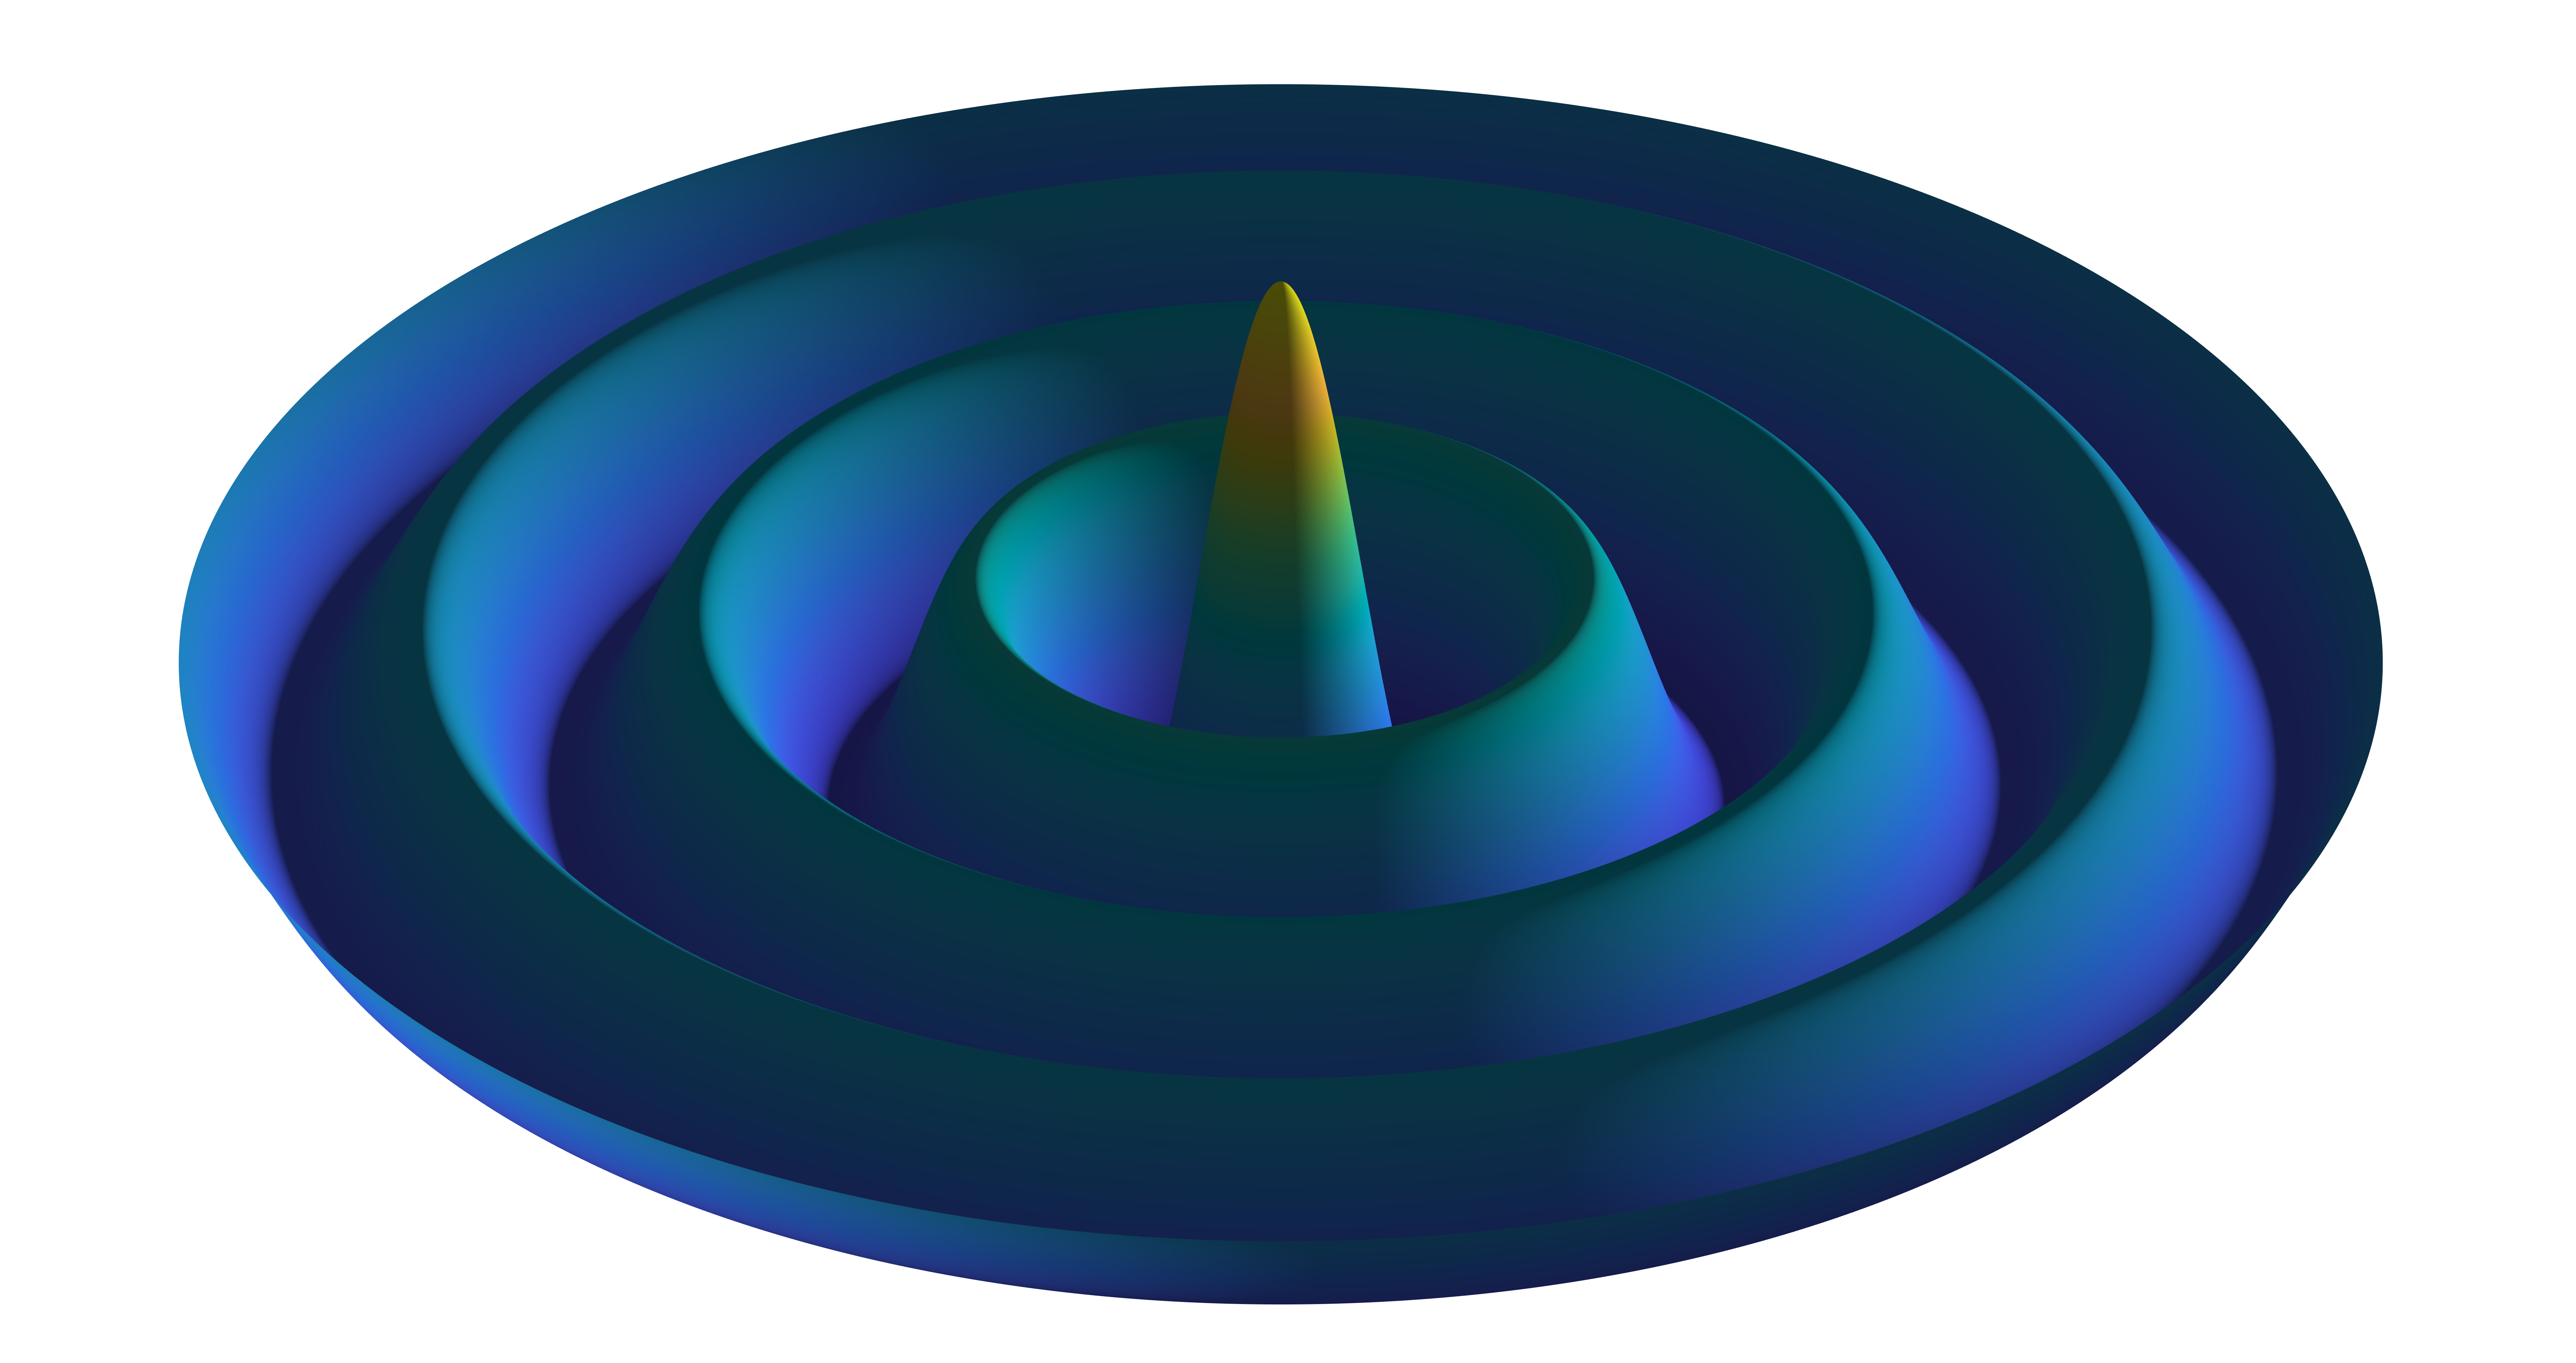
\includegraphics[width=.8\textwidth]{Figures_Part_5/bessel_surface.png}
            \caption{The graph of a radial Bessel function $J_0(\rho)$ where $\rho = \sqrt{x^2+y^2}$. This is a surface whose height is the value of $J_0(\rho)$. This function can be used to describe ripples of water.}
        \end{figure}
        
        \item Functions of the form
        \[
        \vecfieldV \colon \R^3 \to \R^3
        \]
        are called \boldgreen{vector fields}.  Roughly speaking, at each point $\vecx \in \R^3$, we can place a vector $\vecfieldV(\vecx)$ that is also in $\R^3$.  These fields are very important in describing systems that have directional flow.  For example, fluid flow, deformation, and electromagnetism are vector field theories. 

        Vector fields can also be defined on regions $\Omega$ in space or in lower or dimensional settings. Visualization of 2-dimensional vector fields is easiest, but we lose out on lots of more interesting configurations and applications. 

        \begin{figure}[H]
            \centering
            \includegraphics[width=.8\textwidth]{Figures_Part_5/vector_field.png}
            \caption{A plot of a vector field using color to help emphasize the magnitude of the vectors at each point. Note the swirling created by the changing direction of the vectors and the spots where the arrows are longer and where they are shorter.}
        \end{figure}
        \end{enumerate}
        
        The notation we use on the types of functions is telling. Curves $\curvegamma$ are indeed vectors; at a time $t$ they tell us the position of a point in space $\curvegamma(t)$. Scalar fields are scalar valued though their input is a vector. So $f(x,y,z)$ is simply a number assigned to a point in space. Finally, a vector field inputs and outputs a vector. At a point $(x,y,z)$ we will place a new vector $\vecfieldV(x,y,z)$.

        \textcolor{red}{We can wrap all of these up in a fluid example. Curves are the trajectories of single particles, scalars describe quantities of fluids (pressure, temp, height), and vectors show the whole group flow}

        
        \section{Curves in space}
        
        Recall that a curve in space is a function of the form
        \[
        \curvegamma \colon \R \to \R^3.
        \]
        We will specify a specific curve by supplying three functions $\gamma_1(t)$, $\gamma_2(t)$, and $\gamma_3(t)$. Specifically, each of these functions $\gamma_i$ is a function $\gamma_i\colon \R \to \R$. So, a curve in 3-dimensions is made up of three single variable functions. Then, we can say that
        \[
        \curvegamma(t)=\begin{pmatrix} \gamma_1(t)\\ \gamma_2(t)\\ \gamma_3(t)\end{pmatrix}.
        \]
       Each $\gamma_i(t)$ (for the values $i=1,2,3$) represents the components of a vector that changes with respect to the variable $t$. Intuitively, we like to think of the components as evolving in time, which is why we make use of the variable $t$. To say this more explicitly, we can write
        \begin{align*}
            &\gamma_1(t) \quad \textrm{the $x$-position of $\gamma$ at time $t$,}\\
            &\gamma_2(t) \quad \textrm{the $y$-position of $\gamma$ at time $t$,}\\
            &\gamma_3(t) \quad \textrm{the $z$-position of $\gamma$ at time $t$.}
        \end{align*}
        
        \begin{ex}{A Planar Curve}{planar_curve}
        	To see an example, let us take a curve $\curvegamma \colon [0,1] \to \R^2$ by defining
        	\[
        	\curvegamma = \begin{pmatrix} t \\ t \end{pmatrix}.
        	\]
        	This gives us the components
        	\[
        	\gamma_1(t) = t \qquad \textrm{and} \qquad \gamma_2(t) = t.
        	\]
        	We can plot this curve in the plane by plotting the vector for each time $t$. This gives us
        	\begin{figure}[H]
        		\centering
        		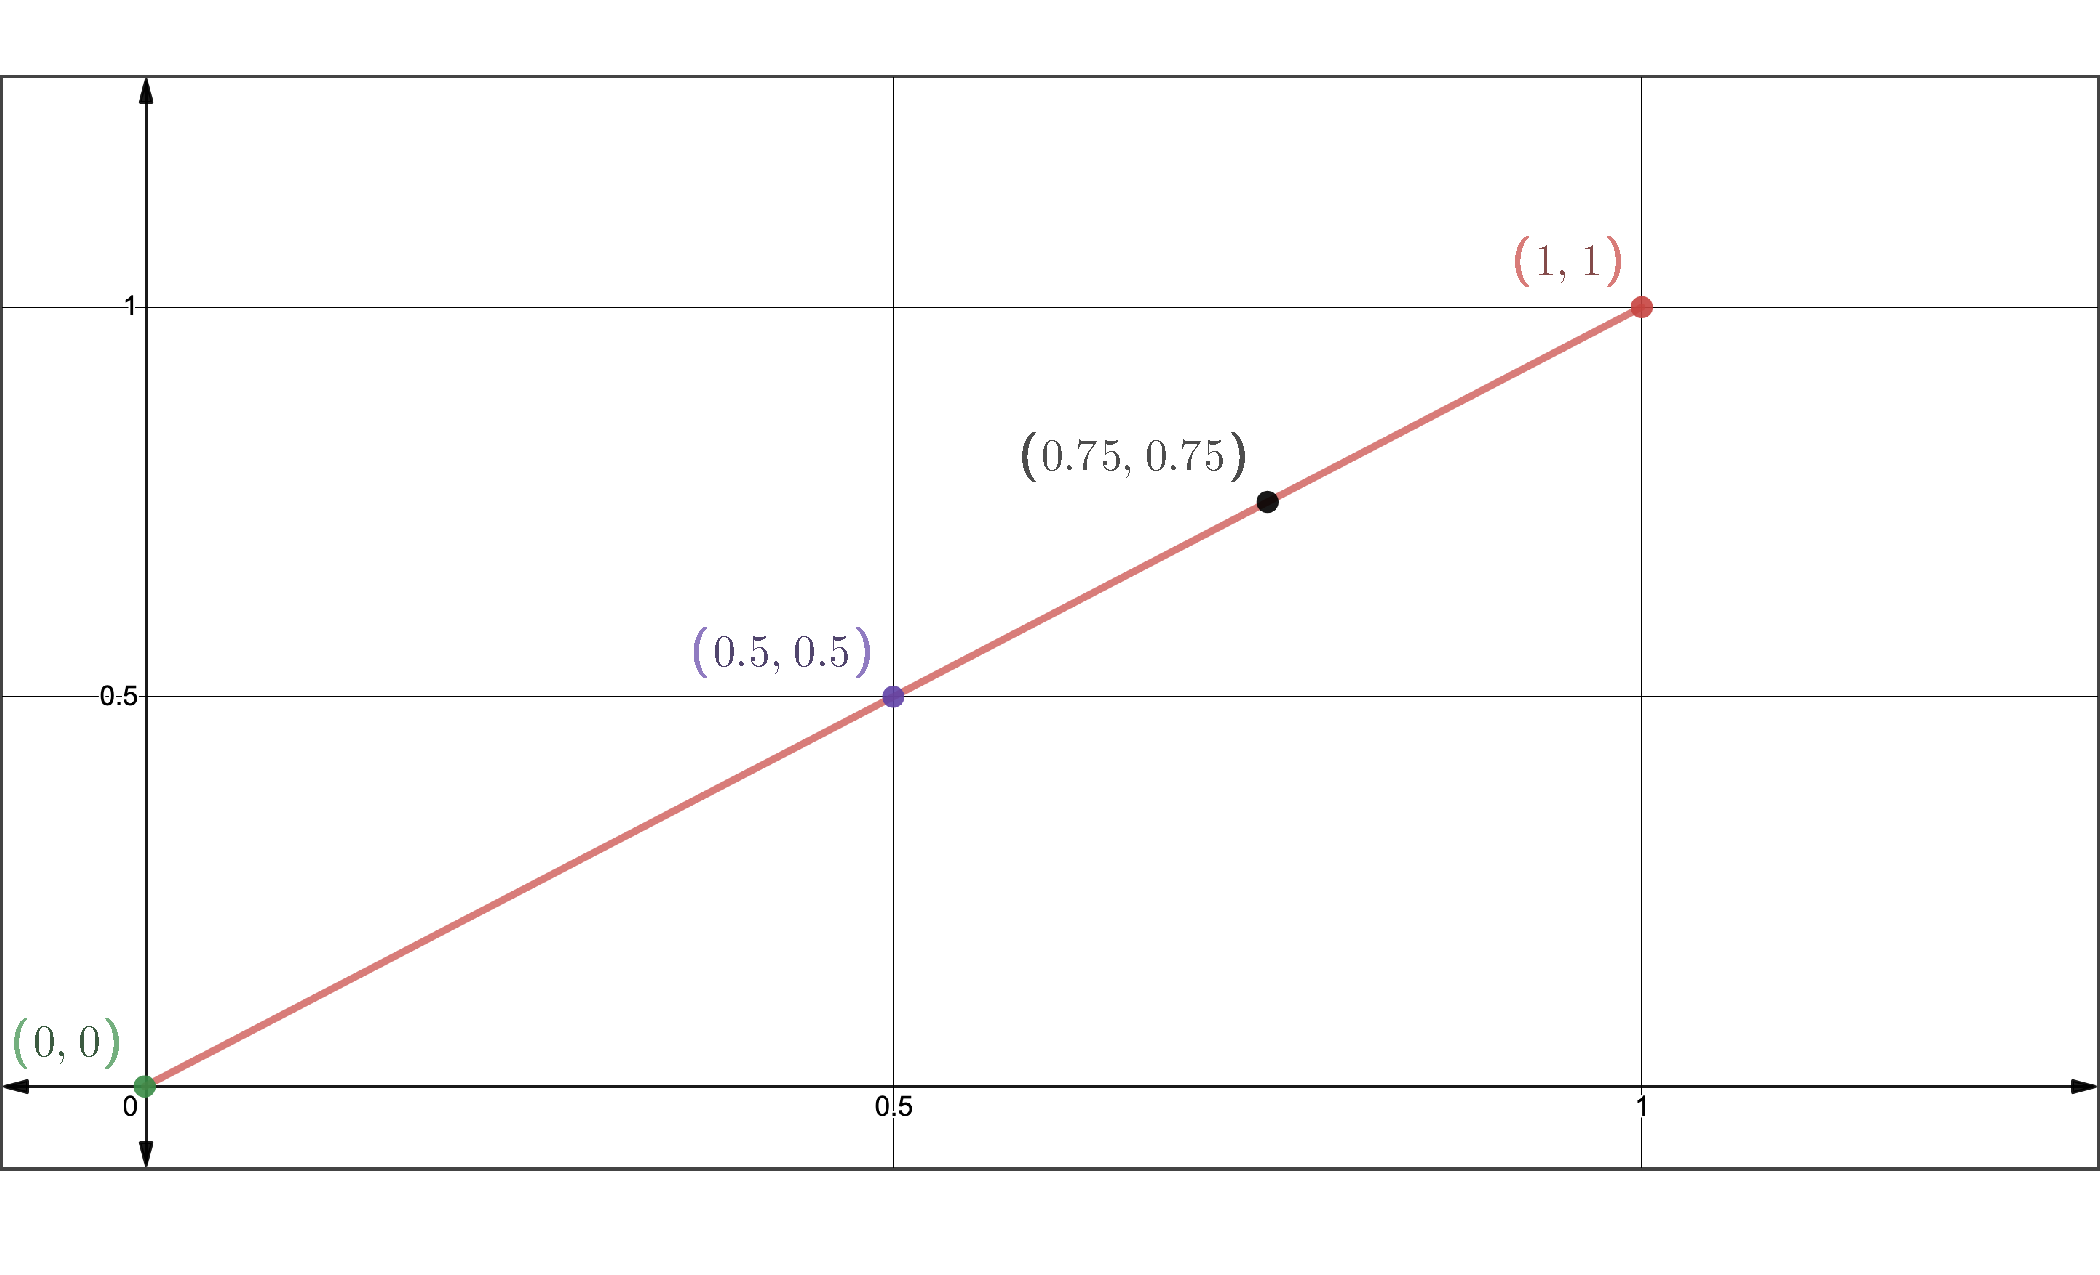
\includegraphics[width=.9\textwidth]{Figures_Part_6/straight_line_curve.pdf}
        		\caption{The curve $\curvegamma(t)$ with labeled points at different times.}
        	\end{figure}
            \textcolor{red}{Replace figure with a color varying curve}
        	In this picture, we can see that the curve begins at the the origin and ends at the point $(1,1)$.  Specifically, we have
        	\[
        	\curvegamma(0) = \begin{pmatrix} 0 \\ 0 \end{pmatrix} \qquad \textrm{and} \qquad \curvegamma(1) = \begin{pmatrix} 1 \\ 1 \end{pmatrix}.
        	\]
        	This curve does not extend indefinitely as our input values can only take on the values in $[0,1]$.
        \end{ex}
        
        From the example, we can see that curves also have a direction associated to them.  As we increase the parameter $t$, we move along the curve in a certain way.  This is an important concept! We can use curves to describe the motion of an object (or other quantities) over time.  This also brings to mind the notion of velocity or speed for a curve.  
        
        \subsection{Derivatives of Curves}
        
        The nice thing about curves is that each component function is a single variable function $\gamma_i\colon \R \to \R$. This means that we can compute the derivatives of each component with the knowledge we have from single variable calculus. In fact, the derivative of a curve can be computed using the typical difference quotient that we learn in a first semester calculus course.  
        
        Imagine that a curve $\curvegamma(t)$ describes the position of a particle at the time $t$.  Then, one could ask for the velocity of this curve which is the first time derivative of position.  Here, we can compute this first derivative at the time $t$ by
        \[
        \tangentgamma(t) = \lim_{\Delta t \to 0} \frac{\curvegamma(t+\Delta t)-\curvegamma(t)}{\Delta t}.
        \]
        We use the overdot notation for $\tangentgamma$ to represent a time derivative of the curve.  We then refer to $\tangentgamma(t)$ as the \boldgreen{tangent} \index{tangent vector} or \boldgreen{velocity vector} \index{velocity vector} to the curve $\curvegamma$ at a time $t$. Now, let us compute the tangent vector explicitly.  We take
        \begin{align*}
        	\tangentgamma(t) &= \lim_{\Delta t \to 0} \frac{\curvegamma(t+\Delta t)-\curvegamma(t)}{\Delta t}\\
        	&= \lim_{\Delta t \to 0} \frac{1}{\Delta t} \left( \begin{pmatrix} \gamma_1(t+\Delta t) \\ \gamma_2(t+\Delta t) \\ \gamma_3(t+\Delta t) \end{pmatrix} - \begin{pmatrix} \gamma_1(t) \\ \gamma_2(t) \\ \gamma_3(t) \end{pmatrix}\right)\\
        	&= \lim_{\Delta t \to 0} \begin{pmatrix} \frac{ \gamma_1(t+\Delta t)-\gamma_1(t)}{\Delta t} \\ \frac{ \gamma_2(t+\Delta t)-\gamma_2(t)}{\Delta t} \\ \frac{ \gamma_3(t+\Delta t)-\gamma_3(t)}{\Delta t} \end{pmatrix}\\
        	&= \begin{pmatrix} \dot{\gamma_1}(t) \\  \dot{\gamma_2}(t) \\ \dot{\gamma_2}(t) \end{pmatrix}.
        \end{align*}
        What this shows is that the tangent vector to a curve $\curvegamma$ is the vector containing the derivative of the components of $\curvegamma$.  Intuitively, this says that the velocity of the curve is found by computing the rate of change of the $x$-component, $y$-component, and $z$-component of $\curvegamma$. 
        
        \begin{ex}{Graph of a Quadratic Function}{graph_quad}
        Consider the curve $\gamma\colon \R \to \R^2$ given by
        \[
        \curvegamma(t)=\begin{pmatrix} t \\ t^2 \end{pmatrix}
        \]
        This curve looks exactly like the graph of the function $f(x)=x^2$ that we have drawn many times before. 
        \begin{figure}[H]
            \centering
            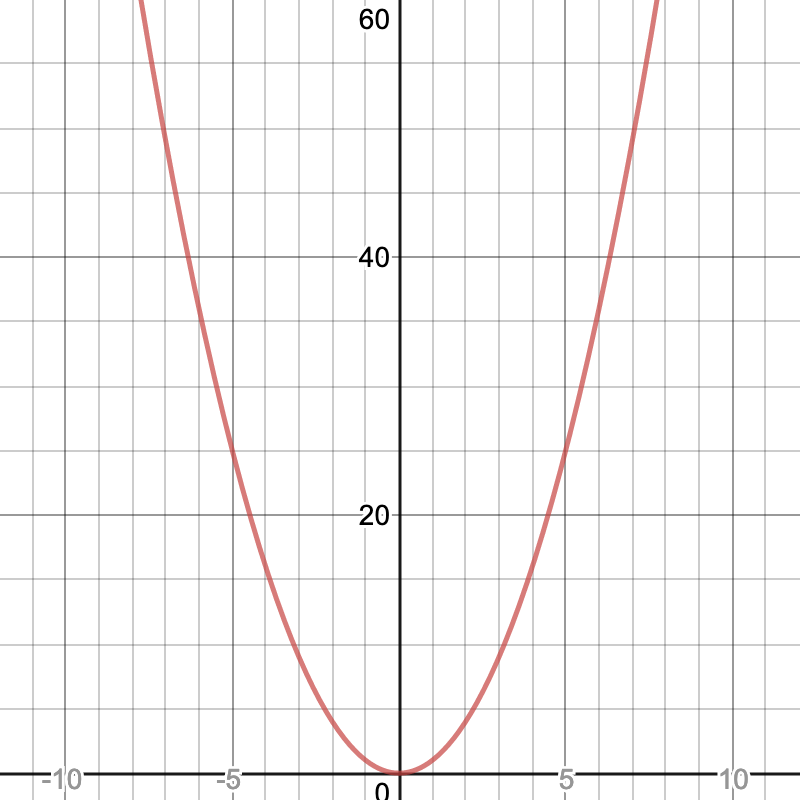
\includegraphics[width=.4\textwidth]{Figures_Part_6/quadratic_curve.png}
        \end{figure}
        What is the tangent vector at time $t$? We have
        \[
        \tangentgamma(t)=\begin{pmatrix} 1 \\ 2t \end{pmatrix}.
        \]
        If we take this $y$-value over the $x$-value we arrive at the same conclusion for the derivative to $f(x)=x^2$ (i.e., $f'(x)=2x$).

        \textcolor{red}{Include better visualization with tangent vectors}
        \end{ex}
        
        The two examples of curves we have seen so far mimic graphs of real valued functions we have seen before.  But, curves can be much more general.  There is no need for a curve to pass the horizontal line test, and curves can even have self intersection! For example, a particle that orbits a large body such as the Earth orbits the Sun will move in an elliptical path.  
        
        \begin{ex}{Circle Curve}{circ_curve}
        Consider the curve $\gamma \colon [0,1] \to \R^2$ given by
        \[
        \curvegamma(t)=\begin{pmatrix} \cos (2\pi t) \\ \sin (2\pi t) \end{pmatrix}.
        \]
        This curve is a circle of radius $1$ centered at $(0,0)$.  We can find the tangent vector at a time $t$ by
        \[
        \curvegamma(t)=\begin{pmatrix} -2\pi \sin(2\pi t) \\ 2\pi \cos(2\pi t)\end{pmatrix}.
        \]
        See the following graphs
        
    \begin{figure}[H]
    \centering
    \begin{subfigure}[h]{0.45\textwidth}
        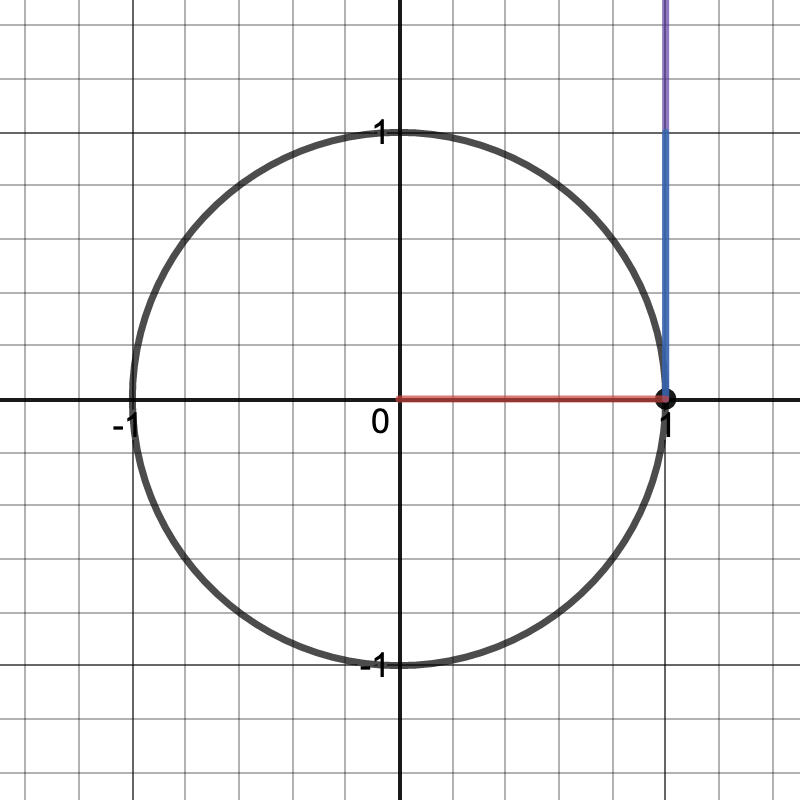
\includegraphics[width=\textwidth]{Figures_Part_6/circ_tang_1.png}
        \caption{Tangent vector at $t=0$.}
    \end{subfigure}
    ~ 
    \begin{subfigure}[h]{0.45\textwidth}
        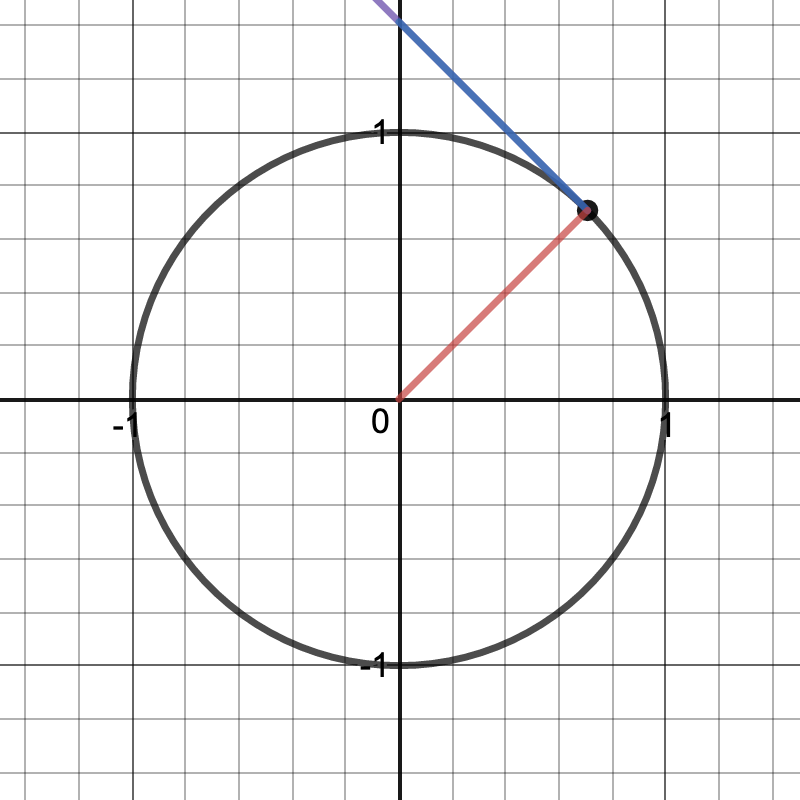
\includegraphics[width=\textwidth]{Figures_Part_6/circ_tang_2.png}
        \caption{Tangent vector at $t=\frac{1}{8}$.}
    \end{subfigure}
    
    \begin{subfigure}[h]{0.45\textwidth}
        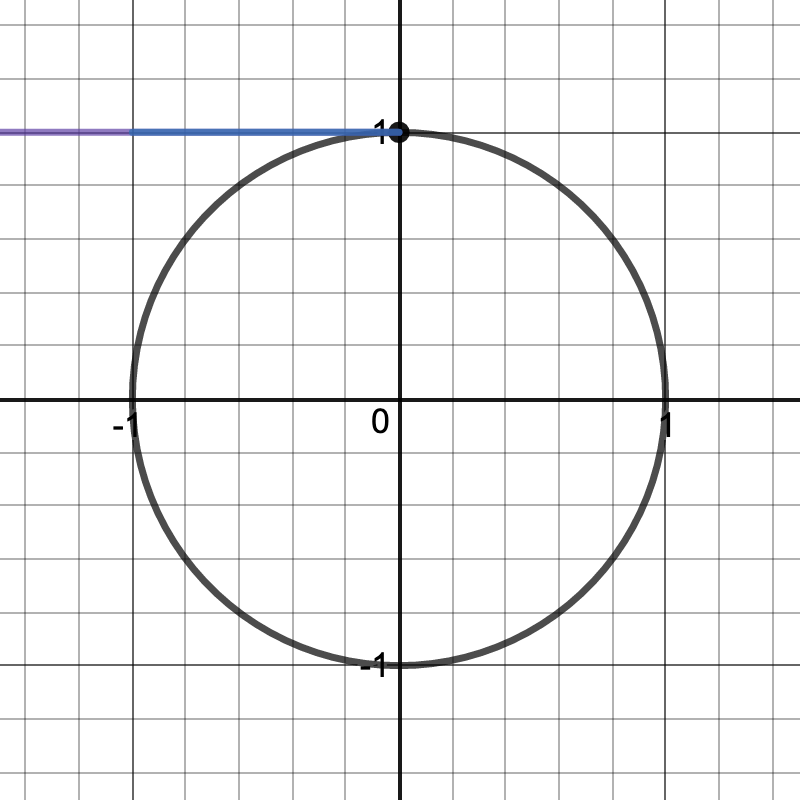
\includegraphics[width=\textwidth]{Figures_Part_6/circ_tang_3.png}
        \caption{Tangent vector at $t=\frac{1}{4}$.}
    \end{subfigure}
    ~
    \begin{subfigure}[h]{0.45\textwidth}
        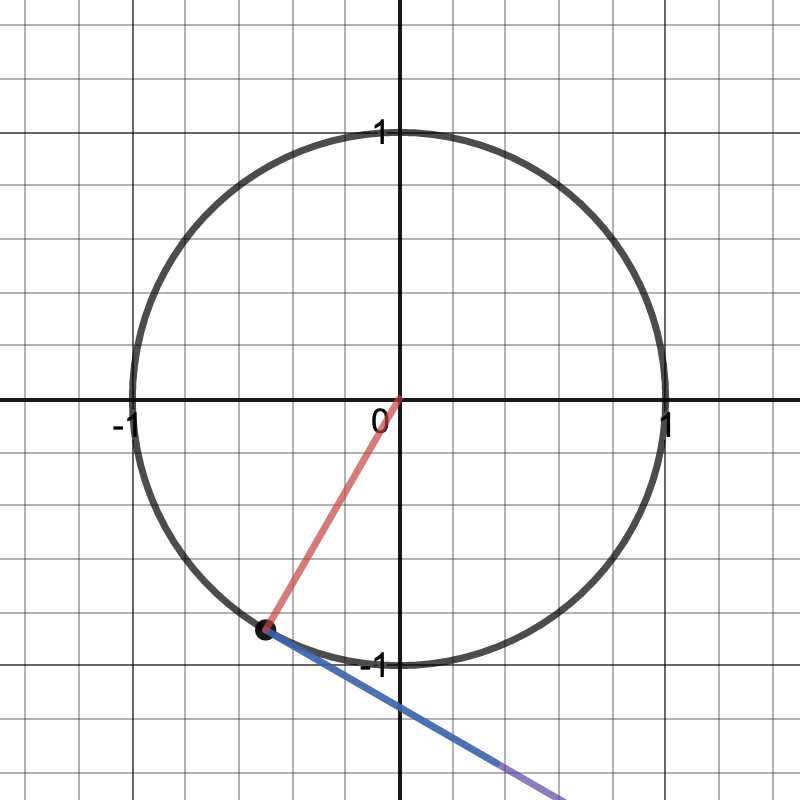
\includegraphics[width=\textwidth]{Figures_Part_6/circ_tang_4.png}
        \caption{Tangent vector at $t=\frac{2}{3}$.}
    \end{subfigure}
        \end{figure}
        \end{ex}
        
        There is nothing stopping us from computing the second time derivative of a curve as well.  We repeat the process for computing the first derivative above, but instead we take the time derivative of the tangent vector $\tangentgamma$.  This yields,
                \[
                \normalgamma(t) = \begin{pmatrix} \ddot{\gamma_1}(t) \\ \ddot{\gamma_2}(t) \\ \ddot{\gamma_3}(t) \end{pmatrix}.
                \]
         We then refer to this quantity as the \boldgreen{normal} \index{normal vector} or \boldgreen{acceleration vector} \index{acceleration vector} to the curve $\curvegamma$. 
         
         \begin{exercise}
         	Compute the normal vector to the circle curve in the previous exercise.  If you know of the notion of centripetal force, how does this quantity relate?
         \end{exercise}
         
         \subsection{Lengths of Curves}
        
        Integration is a tool we use to add up values of functions.  In the 1-dimensional case, we found that the integral of a function $f(x)$ from $x=a$ to $x=b$ computed the net area under the graph of the function.  Similarly, we can use integration to compute the length of a curve.
        
        If we take a curve $\curvegamma \colon [a,b] \to \R^3$, then we can compute the tangent vector at time $t$, $\tangentgamma(t)$. Again, the tangent vector is analogous to the velocity of a curve (at some point in time), and so the length of this tangent vector is the speed.  So, we put that the speed of the curve at time $t$ is $\left| \tangentgamma(t)\right|$. Note that $\left| \tangentgamma(t) \right|$ is a single variable function so we do not need any special tools to integrate this.
        
        Computing the length of a curve amounts to adding up the speed of the curve over the total amount of time.  In this perspective, this just takes into account the total distance a particle has moved, even if the particle back-tracks at some point. We can write this length as
        \[
        \ell(\curvegamma) = \int_a^b \left|\tangentgamma(t)\right|dt.
        \]
        
        \begin{ex}{Circumference of a Circle}{circ_of_circ}
        	Take for example the circle curve $\curvegamma \colon [0,1] \to \R^2$ given by
        	\[
        	\curvegamma(t) = \begin{pmatrix} \cos(2\pi t) \\ \sin(2\pi t) \end{pmatrix}.
        	\]
        	Then, we found 
        	\[
        	\tangentgamma(t) = \begin{pmatrix} -2\pi \sin(2\pi t) \\ 2\pi \cos(2 \pi t) \end{pmatrix}.
        	\]
        	Taking the length of the tangent vector at time $t$ yields
        	\[
        	\left| \tangentgamma(t) \right| = \sqrt{4\pi^2 \sin^2(2\pi t) + 4\pi^2 \cos^2(2\pi t) } = 2\pi.
        	\]
        	The length is then
        	\[
        	\ell(\gamma) = \int_0^1 2 \pi t  = 2\pi,
        	\]
        	which is indeed the circumference of a circle of radius one.
        \end{ex}
                
                \section{Scalar fields}
                The next major class of functions we will consider are the scalar fields.  That is, functions that take the form
                \[
                f\colon \R^3 \to \R.
                \]
                We may also find it helpful to visualize functions by considering instead
                \[
                f\colon \R^2 \to \R
                \]
                and looking at the \boldgreen{graph} of $f$ much like we consider the graph of functions $f\colon \R \to \R$. Let us break down this idea in the 1-dimensional case first.  
                
                \begin{ex}{Graph of a function}{graph_of_func}
                Whenever we talk of a function of the form
                \[
                f\colon \R \to \R
                \]
                we inherently tend to draw the graph of the function $f$.  By graph, I mean that given $f$, we usually just draw the curve $(x,f(x))$ in the plane. Note that this is indeed a curve by the definition we saw prior.
                
                Take for example, $f\colon \R \to \R$ given by $f(x)=x^2$.  We usually draw the plane $\R^2$ and graph the curve $(x,f(x))$ which looks like
                \begin{figure}[H]
                    \centering
                    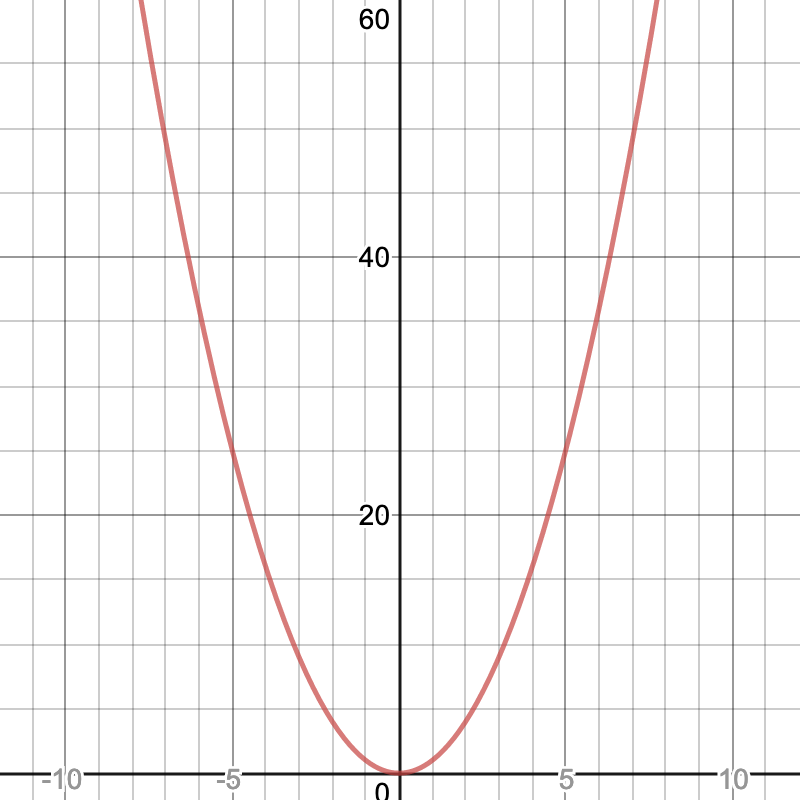
\includegraphics[width=.5\textwidth]{Figures_Part_6/quadratic_curve.png}           
                \end{figure}
                All of this is to say that graphs of these types of functions are special kinds of curves.  In other words, they are curves that pass the vertical line test. 
                \end{ex}
                
                The 1-dimensional examples are rather redundant.  In a vague sense, it can be hard to discern a difference between 1-dimensional curves, scalar fields, and vector fields.  However, if we consider graphing higher dimensional scalar fields, we will immediately see a difference.  Our new point of view will be to look at the graph of 2-dimensional scalar fields in order to gain intuition on the 3-dimensional scalar fields.  
                
                Graphing a 1-dimensional scalar field $f$ involved plotting the graph
                \[
                (x,f(x)).
                \]
                Here, we put the $y$-component of the output as the function $f(x)$ which allows us to see the function values at a point $x$ as the height above (or below) the $x$-axis. Similarly, if we have a scalar field $h(x,y)$, we can plot the set of points
                \[
                (x,y,h(x,y)),
                \]
                in 3-dimensional space.  Then, what we receive is a picture that places $z=h(x,y)$ so that we see the function $h$ describing the height of a rubber sheet above the $xy$-plane. One can imagine that the function $h$ describes how this rubber sheet is deformed. This graph is an example of a \emph{surface} which we will discuss later in this text.
                
                \begin{ex}{The Paraboloid}{paraboloid}
                Let $h\colon \R^2 \to \R$ be given by
                \[
                h(x,y)=x^2+y^2.
                \]
                We can plot the graph of the function by plotting $(x,y, h(x,y))$ in $\R^3$.  This will look like:
                \begin{figure}[H]
                    \centering
                    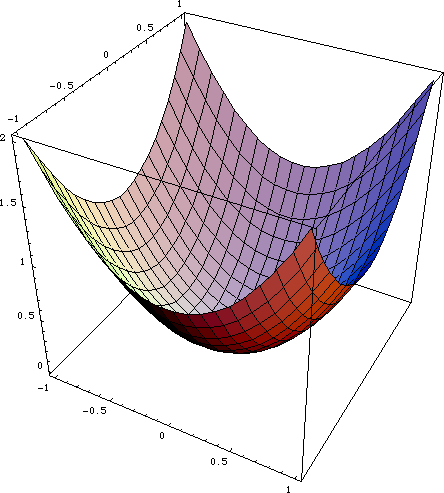
\includegraphics[width=.4\textwidth]{Figures_Part_6/paraboloid.png}
                \end{figure}
                Then we can analyze this function in a few nice ways. For example, if we fix a value for $x$ or $y$, then we will be able to look at $h$ as a function of just a single variable. This will also give us a cross section of the graph. We can imagine that, say setting $y=0$ looks at the slice of the graph where $y=0$ and $x$ is allowed to vary.

                \begin{itemize}
                \item Let us take $y=0$, then we have
                \[
                h(x,0)=x^2.
                \]
                So along the $y=0$ line, the function is just the parabola we are used to! Feel free to repeat this for other values of $y$. 
                
                \item Similarly, we can force $x=0$ and arrive at
                \[
                h(0,y)=y^2
                \]
                is also a parabola.  Again, you should repeat this for various values of $x$.
                
                \item But we are not limited to these choices.  We could have chosen $y=5$ and we would have
                \[
                h(x,5)=x^2+25
                \]
                which is a parabola shifted upwards by 25 units.
                
                \item  Again, we could also choose yet another ``slice" of this function and let $x=y$ which would give us
                \[
                h(x,x)=x^2+x^2=2x^2.
                \]
                So, along the $x=y$ line, the parabola is scaled by 2. Any number of options are available to you here.
                \end{itemize}
                \end{ex}

                One other method of analyzing this function would be to find what the \boldgreen{level curves} of this function are.  What is the set of points $(x,y)$ that satisfy the equation $h(x,y)=c$?  We call these level curves much in the way that a topographical map plots curves along the areas with equal height.  For the previous example with $h(x,y)=x^2+y^2$, consider the set of points $(x,y)$ so that $h(x,y)=1.$ This means
                \[
                f(x,y)=1=x^2+y^2.
                \]
                Since we have
                \[
                x^2+y^2=1
                \]
                that means each level curve is a circle! Here is a ``topographical map" for this function (i.e., a plot of the level curves for this paraboloid.)
                \begin{figure}[H]
                    \centering
                    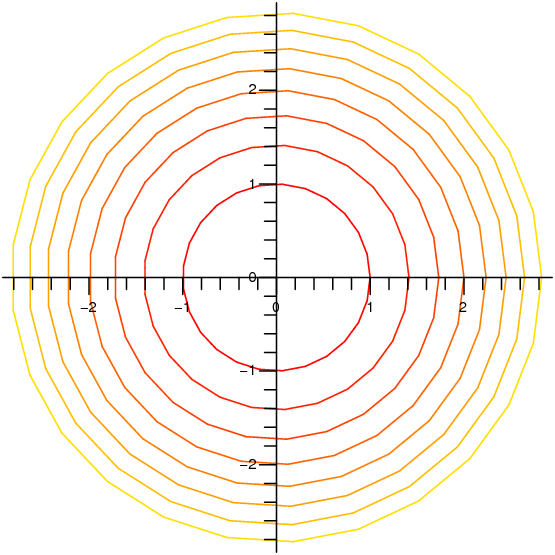
\includegraphics[width=.4\textwidth]{Figures_Part_6/parabolic_level_curves.png}
                \end{figure}
                Here, each circle represents $h(x,y)=c$ for different values of $c$.  This really \emph{is} a topographical map!
                
                
                \begin{exercise}[Plane]
                Repeat this analysis for yourself for the following function:
                \[
                f(x,y)=x+y.
                \]
                \end{exercise}
                
                An important remark is that we should only use this idea to gain intuition. For one, it fails when our function is given by $f\colon \R^n \to \R$ where $n>2$.  The objects for calculus that we develop for scalar fields do not take into account the graph of the function, but just the function itself.  

            \textcolor{red}{Replace previous figures and discuss how coloring can be used to build intuition (based on same idea as level curves)}
                
                \subsection{Partial derivatives of scalar fields}
                       Functions of multiple variables are quite a bit more interesting than their single variable counterparts. As the previous example shows, the visualization becomes more involved and we find that we can, for example, break down the scalar fields into ``slices". This means that we must develop more ways to analyze these higher dimensional functions. 

                        If we take a scalar field $f(x,y,z)$, then we can investigate the rate of change that this function incurs in all possible directions. This of course brings us to the notion of taking derivatives. In particular, we will take derivatives with respect to the individual input variables.
                        
                        \begin{df}{Partial Derivatives}{partial_derivs}
                        Let $f\colon \R^3 \to \R$ be a scalar field.  We define the \boldgreen{partial derivative with respect to $x$} \boldgreen{at the point $(x_0,y_0,z_0)$}, denoted $\frac{\partial f}{\partial x}(x_0,y_0,z_0)$, and put
                        \[
                        \frac{\partial f}{\partial x}(x_0,y_0,z_0)\coloneqq \lim_{\delta \to 0} \frac{f(x_0+\delta,y_0,z_0)-f(x_0,y_0,z_0)}{\delta}
                        \]
                        \end{df}                        
                        
                        \begin{remark}
                        For partial derivatives, all but one variable are being held constant.  So, when you are computing these, be sure to treat the proper variables as constant when necessary.
                        \end{remark}
                        
                        To make notation easier to deal with, we will often just write 
                        \[
                        \frac{\partial f}{\partial x}
                        \]
                        in place of
                        \[
                        \frac{\partial f}{\partial x}(x,y,z).
                        \]
                        When we specify a point at which this partial derivative should be computed, then we must use the notation
                        \[
                         \frac{\partial f}{\partial x}(x_0,y_0,z_0),
                        \]
                        so that the meaning is unambiguous. This definition is readily extended to the other input variables.
                        
                        \begin{exercise}
                        Define $\frac{\partial f}{\partial y}$ and $\frac{\partial f}{\partial z}$ in a similar way to the above definition.
                        \end{exercise}

                        \begin{ex}{Computing partial derivatives}{ex:computing_partials}
                            Consider again the function $h(x,y)=x^2+y^2$ which we analyzed in depth earlier. Then, we can compute the partial $x$ and partial $y$ derivatives. 

                            To compute $\frac{\partial h}{\partial x}$, we will hold the variable $y$ constant and take the derivative of $h$ with respect to $h$. Thus, we have
                            \[
                                \frac{\partial h}{\partial x} = 2x.
                            \]
                            Since $y$ was constant, the derivative must be zero. On top of this, we looked at the behavior of $h$ when we held $y$ constant and found that we get a parabolic function. Indeed, the function $f(x)=x^2$ has a derivative $2x$ just like we found $\frac{\partial h}{\partial x}=2x$. The partial derivative is describing the profile of the graph of $h$ when $y$ is held constant!

                            We repeat this but with respect to the input variable $y$ now. Thus,
                            \[
                            \frac{\partial h}{\partial y} = 2y
                            \]
                            since $x$ is treated as a constant. Once again, we see the function $h(x,y)$ looks like a parabola as we slice along constant values of $x$!
                        \end{ex}
                            
                        
                        \begin{exercise}
                        Compute $\partialx$, $\partialy$, and $\partialz$ for the function 
                        \[
                        f(x,y,z)=\sin(xyz)+x+2y^2+3x^2z.
                        \]
                        \end{exercise}
                        
                        How about second partial derivatives? What can we say here. We have each of the following for a function $f(x,y)$:
                        \begin{itemize}
                            \item $\frac{\partial^2 f}{\partial x^2}$
                            \item $\frac{\partial^2 f}{\partial y^2}$
                            \item $\frac{\partial}{\partial y}\frac{\partial f}{\partial x}$
                            \item $\frac{\partial}{\partial x}\frac{\partial f}{\partial y}$
                        \end{itemize}
                        
                        Recall what $\frac{d^2 f}{dx^2}$ meant for a function $f(x)$.  This told us how $f$ was curving (or what concavity $f$ had). The story is similar for these partial derivatives.
                        
                        \begin{itemize}
                            \item $\frac{\partial^2 f}{\partial x^2}$ tells us about the concavity (or curvature) of $f$ as we move in the $x$ direction.
                            \item $\frac{\partial^2 f}{\partial y^2}$ tells us about the concavity (or curvature) of $f$ as we move in the $y$ direction.
                            \item For nice functions, we actually have that $\frac{\partial}{\partial y}\frac{\partial f}{\partial x}=\frac{\partial}{\partial x}\frac{\partial f}{\partial y}$.  This interpretation is a bit harder to deal with.  Let us not worry too much about it at the moment. We call a second partial derivative of this type a \boldgreen{mixed partial derivative}.
                        \end{itemize}
                        
                        \begin{prop}{Partial Derivatives Commute}{partials_commute}
                        Let $f \colon \R^n \to \R$ be a scalar field with input variables $x_1,x_2,\dots,x_n$. Then if all second partial derivatives of $f$ are continuous, we have that
                        \[
                        \frac{\partial}{\partial x_i}\frac{\partial f}{\partial x_j}=\frac{\partial}{\partial x_j}\frac{\partial f}{\partial x_i},
                        \]
                        for any $i$ and $j$.
                        \end{prop}

                        The interpretation of the proposition is that for sufficiently nice functions (functions whose second partial derivatives are all continuous), the order in which we take the partial derivatives does not matter. So, for example, if we have a 2-dimensional scalar field $f(x,y)$ with continuous second partial derivatives, it must be that
                        \[
\frac{\partial}{\partial y}\frac{\partial f}{\partial x}=\frac{\partial}{\partial x}\frac{\partial f}{\partial y}.
                        \]
                    
                        
                        \begin{exercise}
                        Given $f(x,y)=x^2+y^2$, compute
                        \[
                        \frac{\partial^2 f}{\partial x^2}, \quad \frac{\partial^2 f}{\partial y^2}, \quad \frac{\partial}{\partial y}\frac{\partial f}{\partial x},\quad \frac{\partial}{\partial x}\frac{\partial f}{\partial y}.
                        \]
                        Show through explicit computation that the mixed partial derivatives are equal. What can we say about the curvature of $f$ in the two directions? Does this make sense?
                        \end{exercise}

                \subsubsection{Properties of partial derivatives}
                         
                        As with the one-dimensional derivative, we have some properties that will be helpful.\\
                        
                        \noindent\textbf{Partial Derivatives:}
                        \begin{enumerate}[(i)]
                            \item \textbf{Sum Rule:} Given $f(x,y,z)$ and $g(x,y,z)$, we have that
                            \[
                            \frac{\partial}{\partial x} (f(x,y,z)+g(x,y,z))=\partialx + \frac{\partial g}{\partial x}.
                            \]
                            Of course, this holds for any partial derivative.
                            \item \textbf{Constant Multiple:} Given $\lambda \in \R$ and $f(x,y,z)$, we have that
                            \[
                            \frac{\partial}{\partial x}(\lambda f(x,y,z))=\lambda \partialx.
                            \]
                            Again, this holds for any partial derivative.
                            \item \textbf{Product Rule:} Given $f(x,y,z)$ and $g(x,y,z)$ we have that
                            \[
                            \frac{\partial }{\partial x}(f(x,y,z)g(x,y,z))=\partialx g + f \frac{\partial g}{\partial x}.
                            \]
                            Ths holds for all partial derivatives.
                        \end{enumerate}
                        
                        \begin{remark}
                        The chain rule will show up eventually, but not yet.  As for the quotient rule, this also holds, but I don't show it here.
                        \end{remark}
                        
                        We've learned how to compute partial derivatives and the gradient, but what are they really telling us? Remember that the derivative $\frac{d}{dx}$ of a function $f(x)$ tells us the rate of change of $f$ as we move in the $x$-direction.  This is very similar to what $\frac{\partial}{\partial x}$ tells us about a function $f(x,y,z)$.  So we can say the following.
                        \begin{itemize}
                            \item $\frac{\partial f}{\partial x}$ tells us how $f$ changes as we move in the $x$-direction.
                            \item $\frac{\partial f}{\partial y}$ tells us how $f$ changes as we move in the $y$-direction.
                            \item $\frac{\partial f}{\partial z}$ tells us how $f$ changes as we move in the $z$-direction.
                        \end{itemize}   
                        
                        \subsection{Directional Derivatives}
                        
                        We are not just limited to taking derivatives of scalar fields with respect to the chosen input variables. Much like we can slice up a scalar field in any direction we would like, we can take derivatives of a scalar field in any direction that we would like. Let us take a scalar field $f \colon \R^3 \to \R$ with input $\vecx = (x,y,z)$. Recall that a unit vector $\unitvec$ has length $|\unitvec|=1$. Every unit vector corresponds to a direction in space, and as such allows us to define the \boldgreen{directional derivative} \index{directional derivative}
\[
\frac{\partial f}{\partial \unitvec} \coloneqq \lim_{\delta \to 0} \frac{f(\vecx+\delta \unitvec)-f(\vecx)}{\delta}.
\]
                This derivative then tells us the rate of change of the scalar field $f$ in the direction $\unitvec$. In particular, if we choose a specific point $\vecx_0 = (x_0,y_0,z_0)$, then $\frac{\partial f}{\partial \unitvec}(\vecx_0)$ is the rate of change of $f$ in the direction of $\unitvec$ at the point $\vecx_0$. We will return to this notion later to determine a more simplistic manner in computing this derivative.

                                              
                \section{Vector Fields}
                
                The final object in our new set of functions and fields are the vector fields. Succinctly, a vector field is a function that inputs a vector and outputs a vector. For a vector field in 3-dimensional space $\vecfieldV \colon \R^3 \to \R^3$ we can write
                \[
                \vecfieldV(x,y,z)=\begin{pmatrix} V_1(x,y,z)\\ V_2(x,y,z) \\ V_3(x,y,z)\end{pmatrix}.
                \]
                Try to notice the differences and similarities between vector fields, scalar fields, and curves.  For one, we can see that a vector field is made up of a multiple scalar fields and in this particular instance, we have that $\vecfieldV$ has three scalar field components.  Just as before, it will be nice to visualize many vector fields in the $xy$-plane to avoid drawing in 3-dimensions. Of course, we can use technology to make nice plots in space. Intuitively, one should imagine that a vector field assigns an arrow at each point in space (or at each point on the domain).  This gives us a simple (but tedious by hand) method of visualization.
                
                \begin{ex}{Constant eastward wind}{east_wind}
                Let us define a planar vector field
                \[
                \vecfieldV\colon \R^2 \to \R^2
                \]
                by
                \[
                \vecfieldV(x,y)=\begin{pmatrix} 1 \\ 0 \end{pmatrix}.
                \]
                In this example, the components are $V_1(x,y)=1$ and $V_2(x,y)=0$. At each point $(x,y)$, we are assigning a vector that points a distance 1 in the $x$-direction. This leads us to the following figure.
                \begin{figure}[H]
                    \centering
                    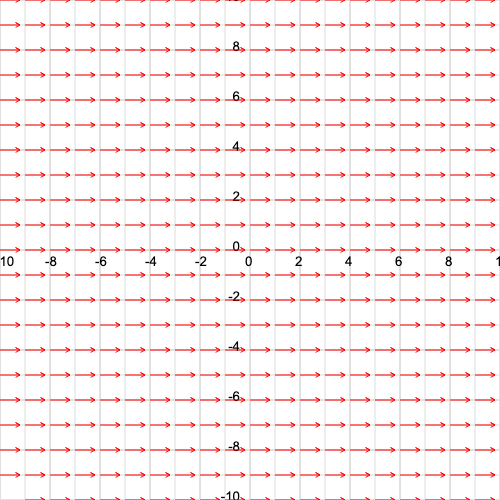
\includegraphics[width=.6\textwidth]{Figures_Part_6/wind_field.png}
                \end{figure}

                To start drawing these fields by hand, the task is as follows:
                \begin{enumerate}[1.]
                    \item Pick a point $(x_0,y_0)$ and evaluate $\vecfieldV(x_0,y_0)$ to get a vector. 
                    \item Take that output vector and attach the tail of that vector at the point $(x_0,y_0)$ in space.
                    \item Repeat steps 1 and 2 until you are satisfied with the illustration you have.
                \end{enumerate}

                The figure in this example took the set of points $(x_0,y_0)$ where $x_0$ and $y_0$ were all integers from $-10$ to $10$. Then, the program computed the output vector at each of those points and glued the tails to those points. One could instead pick different points to draw these arrows at and one can also ``scale" the lengths of the arrows to look nicer since the qualitative look of the vector field is often the most dominant bit of information.
                \end{ex}

                The vector field in the previous example was constant. As the name suggests, one can imagine this as a constant eastward wind. This way of thinking can help one develop an intuition for why we study vector fields in the first place. Fluid motion (such as motion of the atmosphere) is just one prototypical example that we tend to identify with. Challenge yourself to think of other scenarios you have experienced.

                \begin{exercise}
                    Think of the map of the world with a large category five hurricane present in the south Atlantic. Draw a vector field that describes what the wind motion would look like in that case. 
                \end{exercise}

We should not limit ourselves solely with macroscopic fields that we can feel blowing against us. The physical world is field with vector fields that create other dynamics that we see. Atoms and molecules predominantly interact due to their construction from charged particles. These charged particles move due to the electromagnetic field. We will discuss this field later. For now, let us just see more examples.
                
                \begin{ex}{Line source}{line_source}
                Consider the vector field in the plane given by
                \[
                \vecfieldV(x,y)=\begin{pmatrix} x + y\\ x+y \end{pmatrix}.
                \]
                See the following figure.
                \begin{figure}[H]
                    \centering
                    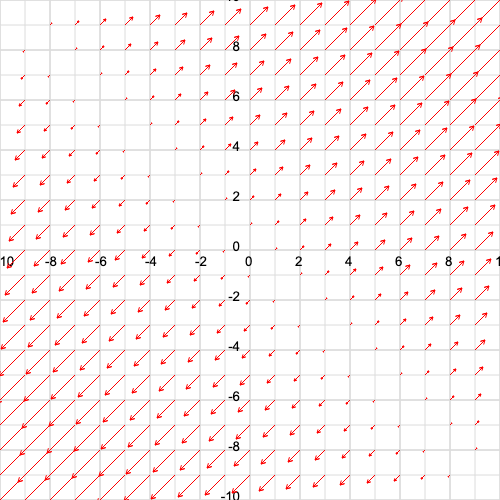
\includegraphics[width=.6\textwidth]{Figures_Part_6/v_field_1.png}
                \end{figure}
                This vector field is zero when $y=-x$. So, along this line, we see no arrows. As we move away from this line, the arrows increase in length and each arrow is pointing in a direction perpendicular to the line $y=-x$. 
                \end{ex}
                
                \begin{ex}{Vortex}{vortex}
                Consider the vector field in the plane given by
                \[
                \vecfieldV(x,y)=\begin{pmatrix} y \\ -x \end{pmatrix}.
                \]
                See the following figure.
                \begin{figure}[H]
                    \centering
                    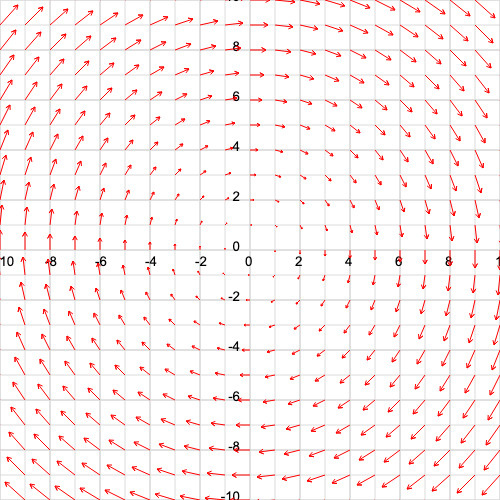
\includegraphics[width=.6\textwidth]{Figures_Part_6/v_field_3.png}
                \end{figure}
                Perhaps this field starts to make you think of a swirling hurricane. In this case, the field seems to swirl in a clockwise direction and as we move further away from the origin, the lengths of each vector increases.
                \end{ex}    
        
        
        
        \subsection{Vector field algebra}
        In our world, we often care about combining different fields together.  For example, we can take the electric field created by a single charged particle and add this field to another field created by a different charged particle. What I mean, is we can write
        \[
        \vecfieldV(x,y,z)+\vecfieldU(x,y,z)
        \]
        and make sense of this.  Just as we did with vectors, we add the components together! That is if we have
        \begin{align*}
        \mathbf{v}(x,y,z)&=(f_1(x,y,z),f_2(x,y,z),f_3(x,y,z))\\ \mathbf{u}(x,y,z)&=(g_1(x,y,z),g_2(x,y,z),g_3(x,y,z)),
        \end{align*}
        then
        \[
        \mathbf{v}(x,y,z)+\mathbf{u}(x,y,z)=(f_1+g_1,f_2+g_2,f_3+g_3).
        \]
        Intuitively, this just adds together the vectors at each point!
        
        \begin{ex}{Addition of vector fields}{add_vect_fields}
        Consider the following vector fields
        \begin{align*}
            \mathbf{v}(x,y)&=(x,x)\\
            \mathbf{u}(x,y)&=(y,y).
        \end{align*}
        These look like:
        \begin{figure}[H]
            \centering
            \begin{subfigure}[h]{.45\textwidth}
            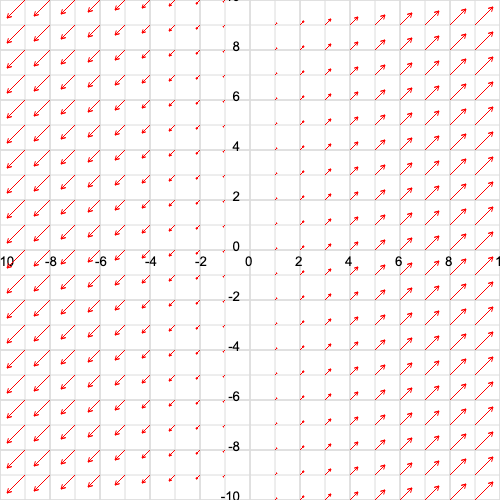
\includegraphics[width=\textwidth]{Figures_Part_6/vec_v.png}
            \caption{Vector field $\mathbf{v}$.}
            \end{subfigure}
            ~
            \begin{subfigure}[h]{.45\textwidth}
            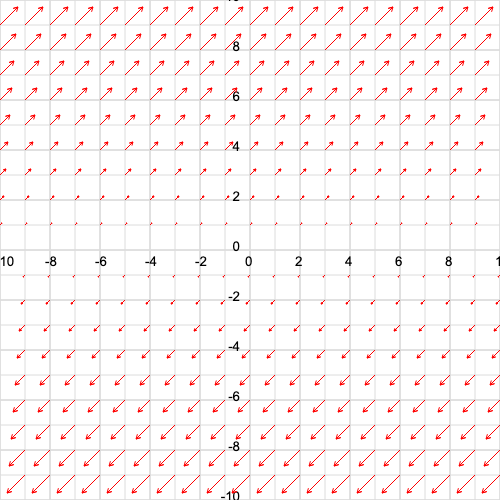
\includegraphics[width=\textwidth]{Figures_Part_6/vec_u.png}
            \caption{Vector field $\mathbf{u}$.}
            \end{subfigure}
        \end{figure}
        Adding these results in the field
        \begin{figure}[H]
            \centering
            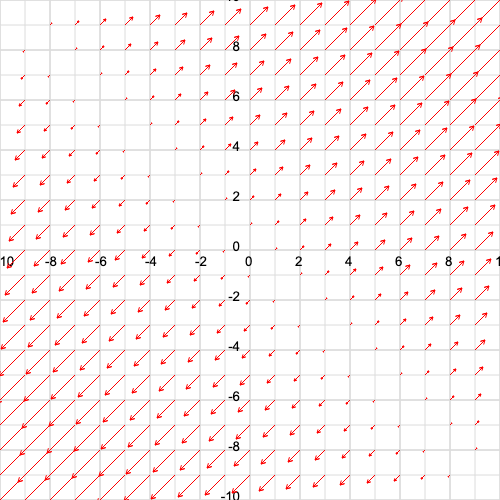
\includegraphics[width=.45\textwidth]{Figures_Part_6/v_field_1.png}
            \caption{The vector field $\vecfieldU+\vecfieldV$.}
        \end{figure}
        \end{ex}
        
        \begin{remark}
        If we do this all for vector fields, we can take curves and scalar fields as special cases.
        \begin{itemize}
            \item Adding together scalar fields is the same as adding functions.  They just have more inputs to think about!
            \item Adding together curves is done in the same componentwise manner that we have shown here for vector fields.
        \end{itemize}
        \end{remark}
        
        We can also scale a field by a real number.  This will stretch vectors at each point.  Just take the vector field
        \[
        \vecfieldV(x,y,z)=\begin{pmatrix} V_1(x,y,z) \\ V_2(x,y,z) \\ V_3(x,y,z)\end{pmatrix}
        \]
        then we can take
        \[
        \lambda \vecfieldV=\begin{pmatrix} \lambda V_1\\ \lambda V_2\\ \lambda V_3\end{pmatrix}.
        \]
        
        In fact, we can scale vector fields by scalar fields! For instance, if we have the scalar field $f(x,y,z)$, then we can create the vector field
        \[
        f(x,y,z) \vecfieldV(x,y,z) = \begin{pmatrix} fV_1 \\ fV_2 \\ fV_3 \end{pmatrix}.
        \]
       This is just computing a scalar multiple of a vector where the scalar is allowed to change from point to point.  For instance, wind flow may also depend on temperature or pressure at that point.
        
        \begin{remark}
        There is many reasons why the above is important.  It seems our physical world plays nicely with the above concept, for one.
        
        One thing we can actually do, and will do a bit later, is find that there are two main types of vector fields in $\R^3$.  These will be the curl fields and divergence fields!  This is important in electromagnetism.
        \end{remark}		        
		        

		        
                      